% CSE 594 Assignment 2 report.  Build:  cd report && tectonic report.tex
% Numbers in macros and \input tables come from ../results/latex/*.tex, written by make_report_assets.py.
% Root-cause counts come from ../results/ft_error_root_causes.csv (hand-labeled).
\documentclass[11pt]{article}
\usepackage[margin=1in]{geometry}
\usepackage[T1]{fontenc}
\usepackage{lmodern}
\usepackage{microtype}
\usepackage{booktabs}
\usepackage{graphicx}
\usepackage{xcolor}
\usepackage{enumitem}
\usepackage{tabularx}
\usepackage{fancyvrb}
\usepackage{float}
\usepackage[most]{tcolorbox}
\usepackage[colorlinks=true,linkcolor=black,citecolor=black,urlcolor=blue!60!black]{hyperref}
\setlist{itemsep=2pt, topsep=4pt}
\setlength{\parskip}{5pt}
\setlength{\parindent}{0pt}
\definecolor{boxgray}{HTML}{F4F4F2}
\newtcolorbox{trialbox}[1]{breakable, colback=boxgray, colframe=black!35, boxrule=0.4pt, arc=2pt,
  left=6pt, right=6pt, top=4pt, bottom=4pt, fonttitle=\bfseries\small, coltitle=black,
  colbacktitle=black!10, title={#1}}
\newcommand{\code}[1]{\texttt{\small #1}}
% Numbered sections print as "Part N: <title>"
\makeatletter
\renewcommand{\@seccntformat}[1]{\ifcsname format@#1\endcsname\csname format@#1\endcsname
  \else\csname the#1\endcsname\quad\fi}
\newcommand{\format@section}{Part~\thesection:\ }
\makeatother

\newcommand{\BaseAccOne}{72.0\%}
\newcommand{\BaseBestOne}{65.5\%}
\newcommand{\BaseComplyOne}{80.5\%}
\newcommand{\BaseFlagRecallOne}{82.8\%}
\newcommand{\BaseFalseAlarmOne}{13.2\%}
\newcommand{\BaseNonePrecOne}{60.6\%}
\newcommand{\BaseNoneRecallOne}{66.7\%}
\newcommand{\BaseInvalidOne}{0}
\newcommand{\BaseErrorsOne}{56}
\newcommand{\FtAccOne}{92.5\%}
\newcommand{\FtBestOne}{86.0\%}
\newcommand{\FtComplyOne}{96.0\%}
\newcommand{\FtFlagRecallOne}{99.2\%}
\newcommand{\FtFalseAlarmOne}{4.9\%}
\newcommand{\FtNonePrecOne}{82.9\%}
\newcommand{\FtNoneRecallOne}{96.7\%}
\newcommand{\FtInvalidOne}{0}
\newcommand{\FtErrorsOne}{15}
\newcommand{\BaseAcc}{72.5\%}
\newcommand{\BaseBest}{66.5\%}
\newcommand{\BaseComply}{81.0\%}
\newcommand{\BaseFlagRecall}{86.9\%}
\newcommand{\BaseFalseAlarm}{16.2\%}
\newcommand{\BaseNonePrec}{61.8\%}
\newcommand{\BaseNoneRecall}{70.0\%}
\newcommand{\BaseInvalid}{1}
\newcommand{\BaseErrors}{55}
\newcommand{\BaseAccTemplate}{73.3\%}
\newcommand{\BaseAccNatural}{71.2\%}
\newcommand{\FtAcc}{93.0\%}
\newcommand{\FtBest}{86.5\%}
\newcommand{\FtComply}{95.5\%}
\newcommand{\FtFlagRecall}{99.2\%}
\newcommand{\FtFalseAlarm}{6.4\%}
\newcommand{\FtNonePrec}{82.9\%}
\newcommand{\FtNoneRecall}{96.7\%}
\newcommand{\FtInvalid}{0}
\newcommand{\FtErrors}{14}
\newcommand{\FtAccTemplate}{94.2\%}
\newcommand{\FtAccNatural}{91.2\%}


% links to files in the public repository
\makeatletter\g@addto@macro\UrlBreaks{\do\_}\makeatother
\newcommand{\repourl}{https://github.com/rajdeeepm/ai-car-advisor}
\newcommand{\gh}[2]{\href{\repourl/blob/main/#1}{\code{#2}}}
\newcommand{\ghdir}[2]{\href{\repourl/tree/main/#1}{\code{#2}}}

% let floats share pages with text, and start float-only pages at the top
\renewcommand{\topfraction}{0.9}
\renewcommand{\bottomfraction}{0.8}
\renewcommand{\textfraction}{0.07}
\renewcommand{\floatpagefraction}{0.8}
\makeatletter
\setlength{\@fptop}{0pt}
\setlength{\@fpsep}{12pt}
\makeatother

\title{\textbf{CSE 594 Assignment 2: AI-Assisted Used Car Selection}}
\author{Rajdeep Mukherjee (\texttt{rajdeepm})}
\date{October 2026}

\begin{document}
\maketitle

% ===========================================================================
\section{Identify or design the task}\label{part:task}

\subsection{The task in the real world}

The broad task is to help a person \textbf{buy a car}, or at least make a more concrete,
better-informed choice when looking at several cars under their own constraints and background.
This is a decision many people face, often more than once, and it is expensive, high-stakes and
personal.

Most buyers are not experts. They may not know what resources exist (vehicle history reports,
safety ratings, recall lookups), what the legal and contractual pitfalls are (branded or
``washed'' titles, dealer add-ons and fees that only appear in the fine print, as-is sales), or
what ownership will cost later in maintenance, parts, insurance and warranty coverage. A listing
that looks like a bargain today can be expensive for years. For example, a luxury car that cost
around \$250,000 new in 2016 may sell for \$70,000--80,000 ten years later, but its parts and
specialist service still cost what they did when it was new, which many buyers overlook. Some
listings are simply \emph{too good to be true}: the low price hides flood damage, a rebuilt
odometer or a scam.

So, the job is not a yes/no classification of ``buy this car or not''. It is reasoning over the
buyer's constraints, what they want, need, or may need in the future, and what each listing
actually implies, then turning that into a choice the buyer understands. An AI assistant can do a
large part of the analysis: check each car against every requirement, catch hidden problems, and
explain what a detail means for the buyer now and later. The decision itself stays with the human.

\subsection{Why neither the AI nor the human should do it alone}

\paragraph{Why the human benefits from the AI:}
\begin{itemize}
  \item \textbf{Volume and diligence:} Even a small comparison means many listings, each with a
  dozen fields and a free-text note, checked against several requirements. People under time
  pressure skip checks; the AI checks every one.
  \item \textbf{Arithmetic:} All-in price (price plus fees) against the budget, mileage limits, and
  comparing qualifying cars on two priorities are tedious for people and quick for a model.
  \item \textbf{Knowledge many buyers lack:} Most first-time buyers don't know that a re-registered
  ``clean'' title after a total loss (title washing) or a request for a gift-card deposit are
  well-known warning signs. The AI names them explicitly.
  \item \textbf{Time and anxiety:} Researching a car takes time many people don't have, and buying
  one is stressful. An assistant that has already done the checking lets the buyer spend their
  attention on the decision rather than on the paperwork.
\end{itemize}

\paragraph{Why the human should not hand over the decision:}
\begin{itemize}
  \item \textbf{The AI does not know the person:} It has no inherent understanding of the buyer's
  needs, past experiences, current constraints, tastes, or plans for the future beyond what they
  tell it. For many people, and especially car enthusiasts, buying a car is an intimate decision
  that depends on how a car feels on a test drive, trust in the seller, appetite for risk, and
  preferences that change once they see the options.
  \item \textbf{The AI still makes confident mistakes:} My fine-tuned model is wrong on
  \FtErrors{} of 200 study trials, and its wrong explanations sound exactly as sure as its right
  ones: ``All-in price \$10,199 is over the \$22,500 budget'' (Section~\ref{sec:errors}).
  \item \textbf{People read everyday language well:} Several of the model's errors are
  human-obvious: ``Some silt behind the dash panels from when the river crested'' is flood damage,
  while ``Not a scam, I promise! Happy to meet at the police station'' is a careful seller, not a
  scam.
  \item \textbf{Consequences and accountability:} A wrong choice costs thousands of dollars and
  years of ownership. The person who pays and drives should own the decision.
\end{itemize}
Whether a decision is ultimately ``right'' for a person is subjective. The goal of the assistance
is to equip the buyer with accurate, applicable information so they can make an educated choice,
not to make the choice for them. In short, the AI is a fast, thorough checker that a human should
verify, not an agent that should buy the car.

\subsection{The task}

With the time and resources available for this assignment, I want to study a narrower version of
this task that can be completed in a few minutes and scored objectively:

\begin{quote}
\emph{Given a buyer's description of their situation and four used-car listings, recommend the
listing that best meets the buyer's needs, or None if no listing does.}
\end{quote}

Each trial takes about 2--3 minutes, so a participant can complete 3--4 trials in a 10-minute
session. The buyer description includes an all-in budget, hard requirements (some stated
outright, some only implied by the story, such as ``I never learned to drive stick''), and two
soft priorities. Each listing has the usual structured fields plus a free-text seller note.

What makes it non-trivial is that the decisive information is often not in the structured
fields. A clean-title car whose seller note says it sat in flood water, a dealer whose fine print
adds \$2,000 in mandatory fees, or a seller who wants a gift-card deposit before any viewing all
fail the buyer's requirement that the car be honestly represented. These are exactly the
too-good-to-be-true situations from the real task.

\paragraph{What is in and out of scope:} I have kept the parts of the real task that can be checked
objectively, including: requirements, budget including fees, hidden problems in seller notes, needs implied by
the buyer's story, and trade-offs between qualifying cars. The scored answer is the
requirement-checking decision. I left out long-term ownership-cost estimates (maintenance,
parts, insurance) and live lookups of recalls, safety ratings or dealer reviews; my model does not
browse the web. The subjective side (how the car feels, trust, taste) is intentionally not scored.
In Assignment~3 I will collect it separately: participants' confidence, ``would you actually buy
this?'', and a short reason.

The exact instructions participants will see, what they are given, and a worked example trial are
in the final section, \hyperref[sec:guidelines]{Study guidelines and participant expectations}.

% ===========================================================================
\section{Identify or create a model to provide AI assistance}\label{part:model}

\subsection{Dataset: my own task and dataset (bonus)}\label{sec:data}

File names in this report link to the GitHub repository; the same files are in the
\code{car\_advisor/} folder submitted on Canvas. I designed the task and created all data myself with my generator (\gh{gen_dataset.py}{gen\_dataset.py},
fixed random seeds). No existing dataset was sampled. I considered a public Craigslist used-car
listings dataset (Zenodo record 10457828, \url{https://zenodo.org/records/10457828}) but did not use
its rows, because real listings come without a ground truth for ``which car should this buyer
pick''. The make and model names are real vehicles, offered only in model years they were actually
produced, but every price, mileage figure, seller and note is fictional.
Table~\ref{tab:splits} lists the three splits I generated and what each one is used for; the
reasons for their sizes follow.

\begin{table}[htbp]
\centering
\caption{The three data splits. Each trial has one buyer and four listings.}
\label{tab:splits}
\begin{tabularx}{\linewidth}{lrrX}
\toprule
Split & Trials & Listings & Used for \\
\midrule
Study & 200 & 800 & Evaluation (Part 3) and Assignment 3 user study; excluded from model training and checkpoint selection \\
Training & 1,620 & 6,480 & LoRA fine-tuning \\
Validation & 180 & 720 & Choosing the training checkpoint (lowest validation loss) \\
\bottomrule
\end{tabularx}
\end{table}

\paragraph{Why these sizes:}
\begin{itemize}
  \item \textbf{Study set, 200 trials:} This meets the assignment's minimum and is large enough
  for balanced strata: 30/70/70/30 trials across the four trial types and 40 per buyer type. It
  also matches the Assignment~3 study: with an assumption of approximately 70 classmates doing 3--4 trials each (roughly
  210--280 completed trials), a larger set would leave most trials with no human answers at all.
  \item \textbf{Training and validation, 1,800 trials split 90/10:} I wanted enough examples for
  the model to learn the output format and the checking rules across all buyer types,
  requirements and red-flag kinds, while keeping training to minutes on one GPU. The training set
  uses the same mix of trial types as the study set (35\% trap, 35\% trade-off, 15\% clear, 15\%
  none). The validation loss flattens over the second epoch (Figure~\ref{fig:loss}), which suggests
  more data of the same kind would add little. I did not run a formal data-size ablation.
\end{itemize}

\paragraph{What a trial contains:} Every trial in every split has the same structure
(Table~\ref{tab:record}). Participants and the model only see the input; the structured
requirements and the answer key are hidden and used for scoring. The submitted CSV has one row
per trial with these fields, plus the model's output and its evaluation.

\begin{table}[!t]
\centering
\small
\caption{Contents of one trial.}
\label{tab:record}
\begin{tabularx}{\linewidth}{>{\raggedright\arraybackslash}p{0.16\linewidth}>{\raggedright\arraybackslash}p{0.19\linewidth}X}
\toprule
Part & Field & Description \\
\midrule
Input (shown) & Buyer profile & A first-person story in plain language: who the buyer is, their
all-in budget, their requirements (stated or implied), the honest-representation requirement,
and their two priorities \\
& Listings A--D & Year, make, model, price, mileage, body style, seats, drivetrain, transmission,
fuel economy (mpg), title status, seller type, location, and a free-text seller note \\
\midrule
Hidden: buyer & Buyer type & One of five (first-time, commuter, family, cold-weather,
outdoor/lifestyle) \\
& Budget & All-in limit in dollars, including required fees \\
& Requirements & Automatic, AWD/4WD, maximum miles, minimum seats, body type; each marked
\emph{stated}, \emph{implied}, or not required \\
& Priorities & Two of: lower price, lower mileage, newer year, better fuel economy, in order \\
\midrule
Hidden: listings & Required fees & Dealer fees that must be paid, including those mentioned
only in the note \\
& Violations & Each requirement the listing breaks and where it is visible: in the fields
(\emph{explicit}), only in the buyer's story (\emph{implied}), or only in the seller note
(\emph{note}) \\
\midrule
Hidden: answer key & Feasible options & Listings that meet every requirement \\
& Acceptable choices & Feasible listings not beaten on both priorities, or None \\
& Best choice & The single top pick under a 0.6\,/\,0.4 weighting \\
& Trial type, wording & Clear, trap, trade-off or no suitable car; generated or hand-written \\
\bottomrule
\end{tabularx}
\end{table}

\paragraph{Why is it built it this way:}
\begin{itemize}
  \item \textbf{Generated, not real listings:} Real listings have no ground truth for which car a
  particular buyer should choose. Generating trials gives every trial a known correct answer, lets
  me control difficulty and balance, and avoids scraping listing sites against their terms of use
  or exposing real sellers.
  \item \textbf{Four listings per trial:} Allows for a real comparison with trade-offs, while still
  fitting into 2--3 minutes so participants can do several trials in a 10-minute session.
  \item \textbf{Tempting hidden-problem cars:} A car with a hidden problem always beats every
  qualifying car on the buyer's top priority. Otherwise, it could be ruled out without reading the
  seller note, and the trial would not test the skill that matters most in real car buying.
  \item \textbf{Stated and implied requirements:} Real buyers describe their lives (``my doctor said
  no clutch work for a year''), not checklists. Mixing both forms enables us to test whether the performer
  understands the story rather than matching keywords.
  \item \textbf{The honest-representation requirement:} Every buyer says the car must be honestly
  represented. That makes flood or frame damage, washed titles, unreliable odometers, scams and
  looming major repairs objective deal-breakers instead of matters of taste, so they can be scored.
  \item \textbf{No-suitable-car trials:} Sometimes the right answer is to walk away. These trials
  test whether the performer, or the AI, notices when nothing qualifies, and whether people follow
  an AI that recommends a car anyway.
  \item \textbf{A rule-based answer key:} The correct answer is computed from the structured data,
  not judged by me. It is objective and reproducible, and it scores the AI and human participants
  in exactly the same way.
\end{itemize}

\paragraph{How a trial is built:}
\begin{enumerate}
  \item \textbf{Buyer:} One of five buyer types (first-time buyer, daily commuter, family,
  cold-weather driver, outdoor/lifestyle) sets a budget range (\$7,000--\$36,000) and likely
  requirements. Each requirement is randomly phrased outright or implied in the story. Every buyer
  also states that the car must be honestly represented.
  \item \textbf{Listings:} Cars are sampled from a 38-model catalog with real production years.
  Price is derived from age, mileage and a new-car price, with noise.
  \item \textbf{Roles:} Each listing is assigned a role: \emph{qualifies}, \emph{visible violation}
  (for example over budget or a salvage title), or \emph{hidden problem} (a deal-breaker only in the
  seller note or only implied by the buyer's story). Hidden-problem cars are deliberately tempting:
  they beat every qualifying car on the buyer's top priority.
  \item \textbf{Answer key:} Computed by rule from the trial's structured data
  (Section~\ref{sec:bench} gives the scoring rules).
\end{enumerate}
The generator mixes these roles into four trial types, each testing a different skill
(Table~\ref{tab:composition}). Most of the study set is trap and trade-off trials, because those
are the ones where reading the fine print and weighing priorities matter.

\begin{table}[htbp]
\centering
\caption{Composition of the 200 study trials.}
\label{tab:composition}
\begin{tabularx}{\linewidth}{lrX}
\toprule
Trial type & Trials & What it tests \\
\midrule
Clear & 30 & One qualifying car; every other car fails visibly \\
Trap & 70 & One qualifying car plus a tempting car with a hidden problem \\
Trade-off & 70 & Two or three qualifying cars that trade off the buyer's priorities \\
No suitable car & 30 & Every car fails; the right answer is None \\
\bottomrule
\end{tabularx}
\end{table}

The trials are balanced across the five buyer types (40 each) and the correct letter (A 40, B 44,
C 48, D 38, None 30). In 116 trials at least one listing has a hidden problem. Across all 800
listings there are 122 seller-note deal-breakers: flood damage (16), frame damage (26), washed
title (16), unreliable odometer (17), scam-like payment request (18), major repair needed (14)
and required fees that break the budget (15). There are also 32 implied-need violations.

\paragraph{Separation of datasets:} The training and validation sets come from a different seed. They contain
do not contain any of the study trials, buyer texts or car sets (checked programmatically), and not a single one of the
study-only hand-written phrasings described below.

\paragraph{Dataset iterations:}
\begin{itemize}
  \item \textbf{Iteration 1 to 2: hand-written wording:} In the first version of the study set,
  every seller note and implied need came from the same kinds of templates as the training data.
  The fine-tuned model scored \FtAccOne{} on it, which raised two concerns: the score might reflect
  memorized phrasing rather than understanding, and a near-perfect AI on template text would make
  the task one people should simply delegate. Thus, I rewrote 80 of the 200 study trials
  (40\%, stratified by trial type) with hand-written notes and buyer stories that never appear in
  training: red flags buried in otherwise positive notes, harmless notes with alarming words (``I
  rebuilt the front suspension myself''), and implied needs told as anecdotes. The answer key is
  unchanged, so the two versions are directly comparable (Section~\ref{sec:adjust}). This revision
  was guided by the study-set result, as the assignment's iteration step allows; the model was not
  retrained or tuned in response, and the change made the study set harder for the model, not
  easier.
  \item \textbf{Data realism fix:} While preparing the report I found that the generator could pair
  a model with a year in which it was never made (for example, a 2015 Kia Telluride, which launched
  in 2020). Hence, I added real production-year ranges,
  regenerated all splits from the same seeds, retrained the model and reran every evaluation. All
  numbers in this report are from the regenerated data. The results before the fix were very similar
  (base 72.0\%, fine-tuned 92.5\%), so no conclusion depends on it.
\end{itemize}

\subsection{The AI assistance}\label{sec:assist}

For every trial the model returns JSON with five parts, which the Assignment~3 interface will show
next to the listings:
\begin{enumerate}
  \item \code{option\_checks}: a one-line verdict for each listing (``Fails: required dealer fees
  bring the all-in price to \$19,894, over the \$19,000 budget'').
  \item \code{red\_flags}: problems found in seller notes, with the listing and the issue.
  \item \code{recommendation}: A, B, C, D or NONE.
  \item \code{reason}: why that listing best fits the buyer.
  \item \code{tradeoffs}: what the buyer gives up compared with the other qualifying listings.
\end{enumerate}
The per-listing checks and red flags let a human verify the AI's work quickly instead of taking
the recommendation on trust.

\subsection{The model and why I chose it}

The assistant is \textbf{Qwen3-4B-Instruct-2507} \cite{qwen3}, \textbf{fine-tuned by me with LoRA}
\cite{lora} on my 1,620 training trials. I chose it because:
\begin{itemize}
  \item \textbf{Open weights (Apache-2.0):} I can fine-tune it and host it myself, so the
  Assignment~3 interface can show live AI output instead of copied chat-interface answers.
  \item \textbf{Small enough to train and serve cheaply:} At 4 billion parameters it fine-tunes in
  minutes on one GPU and answers a trial in about a second when batched, which matters for an
  interactive study.
  \item \textbf{Strong instruction following for its size}, including reliable JSON output, and the
  2507 ``Instruct'' variant answers directly without long hidden reasoning traces, which keeps
  responses fast and predictable.
\end{itemize}

\paragraph{Initial performance and why I fine-tuned:} With a careful prompt, the base model chose
an acceptable car on \BaseAcc{} of study trials. Its errors were systematic
(Figure~\ref{fig:errors}a): it often took the tempting car with a hidden problem (it flagged only
\BaseFlagRecall{} of seller-note deal-breakers), picked cars beaten on both priorities, said None
when a car qualified, raised false alarms on \BaseFalseAlarm{} of fully qualifying cars, and once
produced unparseable output. That is likely no better than an attentive person, so it would be
weak assistance. Fine-tuning targets those behaviors: checking every listing against every
requirement, telling deal-breakers from cosmetic issues, and abstaining only when nothing
qualifies.

\paragraph{How I fine-tuned:} Each training example is a buyer profile and four listings (input)
and a reference answer in the same JSON format (target). Reference answers are generated from the
answer key: the true violations of each listing, the hidden red flags, the correct choice, and a
numeric comparison of the qualifying alternatives. I trained with TRL's \code{SFTTrainer}
(\gh{train_lora.py}{train\_lora.py}): LoRA rank 16, alpha 32, dropout 0.05, on all attention and MLP projections
(33M trainable parameters, 0.81\% of the model); 2 epochs, learning rate $10^{-4}$ with cosine
decay and 20 warm-up steps, effective batch size 8, bf16, maximum length 3,072 tokens, loss on the
answer tokens only. The checkpoint with the lowest validation loss is kept; it was the final step
(validation loss 0.006, Figure~\ref{fig:loss}). Inference uses greedy decoding, so outputs are
deterministic, and base and fine-tuned models get the identical system prompt and input.

\begin{figure}[htbp]
\centering
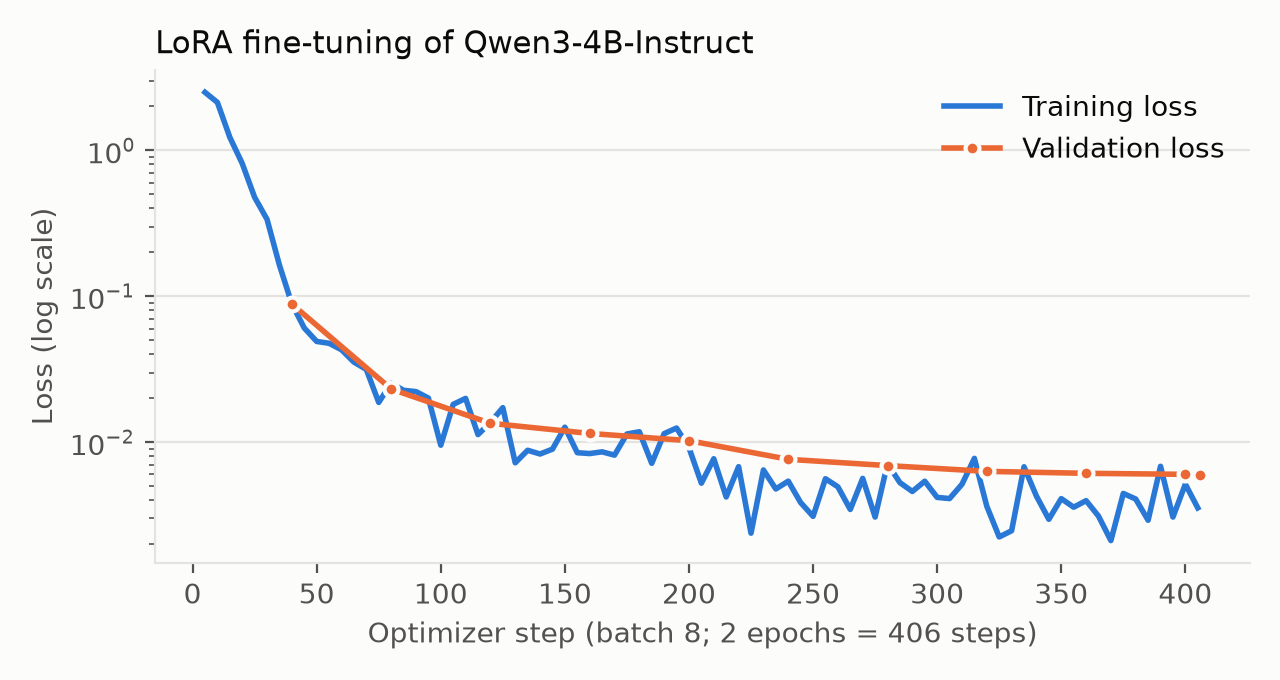
\includegraphics[width=0.74\linewidth]{../results/figures/loss_curve.png}
\caption{Training and validation loss during LoRA fine-tuning (log scale).}
\label{fig:loss}
\end{figure}

\paragraph{What fine-tuning changed:} The acceptable-choice rate rose from \BaseAcc{} to \FtAcc{},
red-flag recall from \BaseFlagRecall{} to \FtFlagRecall{}, and false alarms fell from
\BaseFalseAlarm{} to \FtFalseAlarm{} (full comparison in Section~\ref{sec:results}). Not everything
improved: performance on clear trials did not change, the model scores a few points lower on
hand-written wording than on generated wording, and it became over-cautious, so that wrongly saying
None is now its most common outcome error (Section~\ref{sec:errors}). Figure~\ref{fig:demo} shows the fine-tuned model
running on one study trial, as evidence that it works end to end.

\IfFileExists{figures/demo_screenshot.png}{%
\begin{figure}[p]
\centering
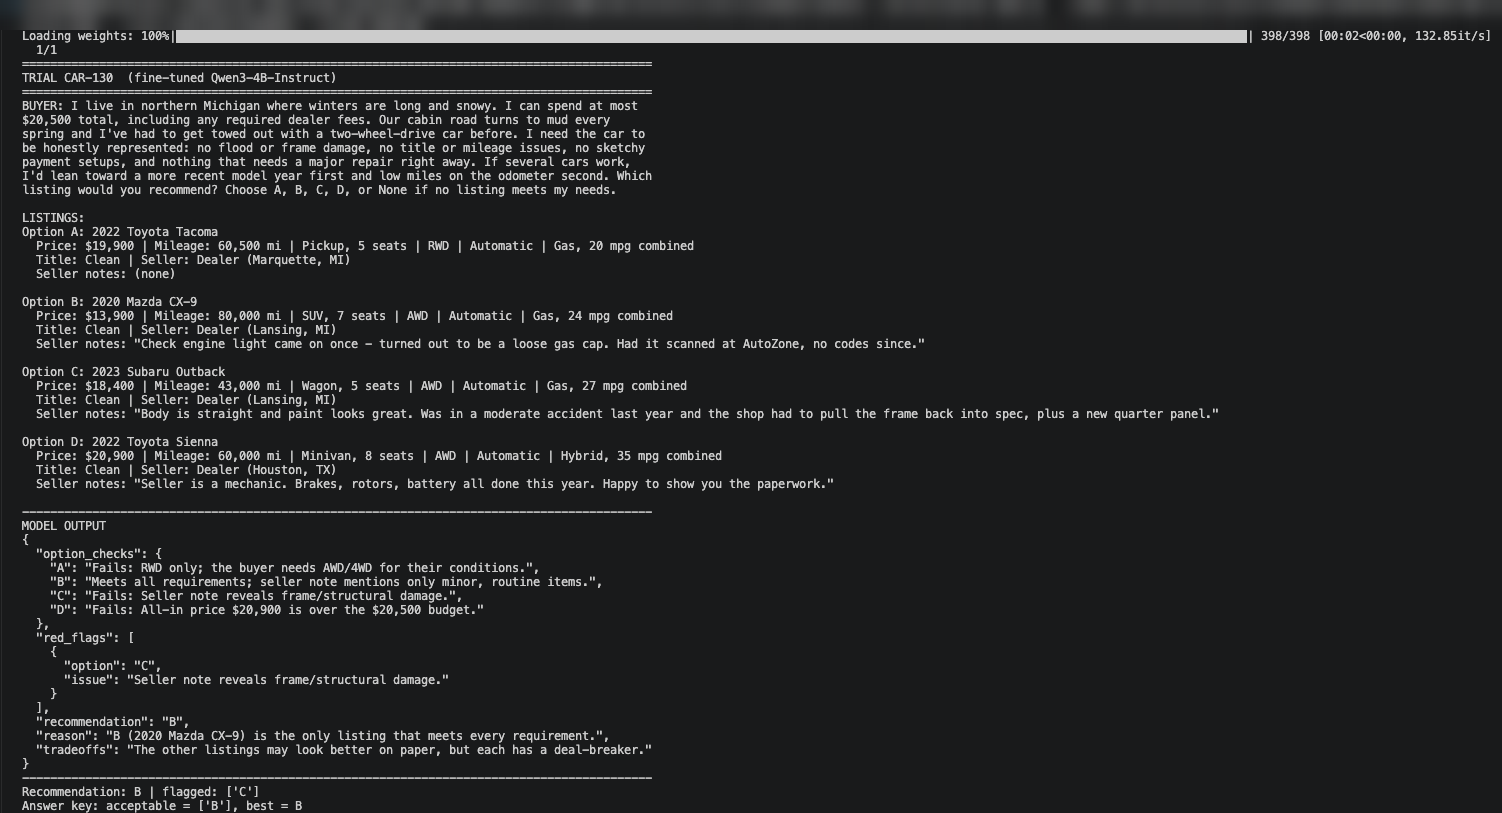
\includegraphics[width=0.9\linewidth]{figures/demo_screenshot.png}

\medskip
\VerbatimInput[fontsize=\tiny,frame=single,framesep=2mm]{demo_output.txt}
\caption{The fine-tuned model on study trial CAR-130 (\gh{demo.py}{demo.py}): screenshot (top, machine
details blurred) and the same output as text (bottom). C hides frame damage in its note, A is
rear-wheel drive (ruled out by the muddy cabin road), and D is \$400 over budget. The model flags
C and recommends B, matching the answer key.}
\label{fig:demo}
\end{figure}}{}

\subsection{Replicating and hosting the model}

\paragraph{What someone would need to do:} The model is not hosted anywhere public, so anyone who
wants to use it runs it on their own machine. The code, data and saved outputs are in the
\code{car\_advisor/} folder submitted on Canvas and in the repository
\url{https://github.com/rajdeeepm/ai-car-advisor}. The trained LoRA adapter is in the repository and in the separate
Canvas file \path{CSE594_A2_car_advisor_adapter.zip}, so retraining is optional. The adapter (130\,MB) is over GitHub's 100\,MB file limit, so it is stored as two zip
parts; \gh{setup.sh}{setup.sh} joins them, checks them against a checksum and unzips the adapter
into \code{model/lora\_adapter/}:
\begin{enumerate}
  \item Get the adapter: unzip \path{CSE594_A2_car_advisor_adapter.zip} in the same folder as
  \path{CSE594_A2_car_advisor_files.zip}, which places it in \path{car_advisor/model/}. Or
  clone the repository and run \code{bash setup.sh}.
  \item Install Python 3.12 with PyTorch 2.13 (CUDA), Transformers 5.17, PEFT 0.21 and TRL 1.15
  (the versions I used; \gh{requirements.txt}{requirements.txt} and the \gh{README.md}{README} list them).
  \item Download the base model from Hugging Face (\href{https://huggingface.co/Qwen/Qwen3-4B-Instruct-2507}{\code{Qwen/Qwen3-4B-Instruct-2507}}, about 8\,GB).
  \item \textbf{To use my model:} run \gh{infer.py}{infer.py} (a whole split) or \gh{demo.py}{demo.py} (one
  trial), passing the adapter folder with the \code{--lora} option. For a live interface, the same loading code can sit behind
  a small web endpoint; a serving engine such as vLLM can make it faster.
  \item \textbf{To retrain it:} regenerate the data with \gh{gen_dataset.py}{gen\_dataset.py} and run
  \gh{train_lora.py}{train\_lora.py}, or run \gh{run_all.sh}{run\_all.sh}, which trains and then produces every prediction
  used in this report.
\end{enumerate}

\paragraph{Resources needed:} One NVIDIA GPU with CUDA. About 24\,GB of GPU memory is enough for
inference. Training also runs on one GPU; on cards with less memory, lower the per-device batch
size and raise gradient accumulation to keep the effective batch at 8 (for example on a Google
Colab A100). About 10\,GB of disk covers the base model, adapter and data.

% ===========================================================================
\section{Evaluate the model}\label{part:eval}

\subsection{Benchmarking: method and metrics}\label{sec:bench}

\paragraph{How I benchmarked the model performance:} Both models, the base Qwen3-4B-Instruct and my fine-tuned version,
answer all 200 study trials with the identical prompt and greedy decoding. Each output is parsed
and scored automatically against a rule-based answer key (\gh{evaluate.py}{evaluate.py}):
\begin{enumerate}
  \item A listing is \textbf{feasible} only if it meets every requirement: the all-in budget (price
  plus required dealer fees), no branded title, any required transmission, drivetrain, seats, body
  type or mileage limit (stated outright or implied in the story), and no deal-breaker in the
  seller note (flood or frame damage, washed title, unreliable odometer, scam-like payment request,
  major repair needed).
  \item If no listing is feasible, the correct answer is \textbf{None}.
  \item Otherwise a choice is \textbf{acceptable} if it is feasible and no other feasible listing is
  at least as good on both of the buyer's stated priorities and strictly better on one (it is
  Pareto-optimal on the two priorities). The single \textbf{best} choice uses a 0.6\,/\,0.4 weighted
  score of the two priorities, each min-max normalized within the trial.
\end{enumerate}
As a sanity check, the reference answers used for training score 100\% under these rules.

\paragraph{Metrics and why I chose them:}
\begin{itemize}
  \item \textbf{Acceptable-choice rate (primary):} A buyer who says ``low miles first, then price''
  has not told me how many dollars a mile is worth, so when two cars each win on one priority,
  either is a defensible recommendation. Scoring only an exact match would penalize reasonable
  answers for my own arbitrary weighting. This is also the metric I will use for humans in
  Assignment~3, so all three conditions are compared on the same scale.
  \item \textbf{Exact best choice (secondary):} Agreement with the 0.6/0.4 weighted pick, reported
  for completeness.
  \item \textbf{Meets all requirements:} The share of trials where the model did \emph{not}
  recommend a car that breaks a hard requirement or wrongly say None. These are the expensive
  errors for a real buyer (a flood car, a scam), as opposed to picking a slightly worse qualifying car.
  \item \textbf{Red-flag recall and false-alarm rate:} The interface shows the AI's red flags, so
  their quality matters on its own: recall is the share of seller-note deal-breakers the model
  flagged; the false-alarm rate is the share of fully qualifying listings it flagged anyway.
  \item \textbf{None precision and recall:} How reliably the model abstains when nothing qualifies,
  and only then.
\end{itemize}

\paragraph{How the metric choice affects the results:} The choice matters most for trade-off
trials. The fine-tuned model's acceptable-choice rate (\FtAcc{}) is higher than its exact-best rate
(\FtBest{}): in the trials in between, it picked a car that is defensible for the buyer but not the
one my particular weighting prefers. Scoring by exact match would make the AI look worse for
reasons a buyer would not care about, and it would make the human--AI comparison in Assignment~3
depend on an arbitrary weighting. The separate red-flag and requirement metrics show \emph{how}
the model is right or wrong, which matters because the interface shows its reasoning, not just its
answer.

\subsection{Results: before and after fine-tuning}\label{sec:results}

\begin{table}[htbp]
\centering
\caption{Base vs.\ fine-tuned model on the final 200-trial study set. $\uparrow$: higher is better; $\downarrow$: lower is better (false alarms and unparseable outputs).}
\label{tab:metrics}
\begin{tabular}{lrr}
\toprule
Metric & Base Qwen3-4B & Fine-tuned (LoRA) \\
\midrule
Acceptable choice, primary ($\uparrow$) & 72.5\% & 93.0\% \\
Exact best choice ($\uparrow$) & 66.5\% & 86.5\% \\
Meets all requirements ($\uparrow$) & 81.0\% & 95.5\% \\
Red-flag recall ($\uparrow$) & 86.9\% & 99.2\% \\
Red-flag false alarms ($\downarrow$) & 16.2\% & 6.4\% \\
None precision ($\uparrow$) & 61.8\% & 82.9\% \\
None recall ($\uparrow$) & 70.0\% & 96.7\% \\
Unparseable outputs ($\downarrow$) & 1 & 0 \\
\bottomrule
\end{tabular}

\end{table}

\begin{figure}[htbp]
\centering
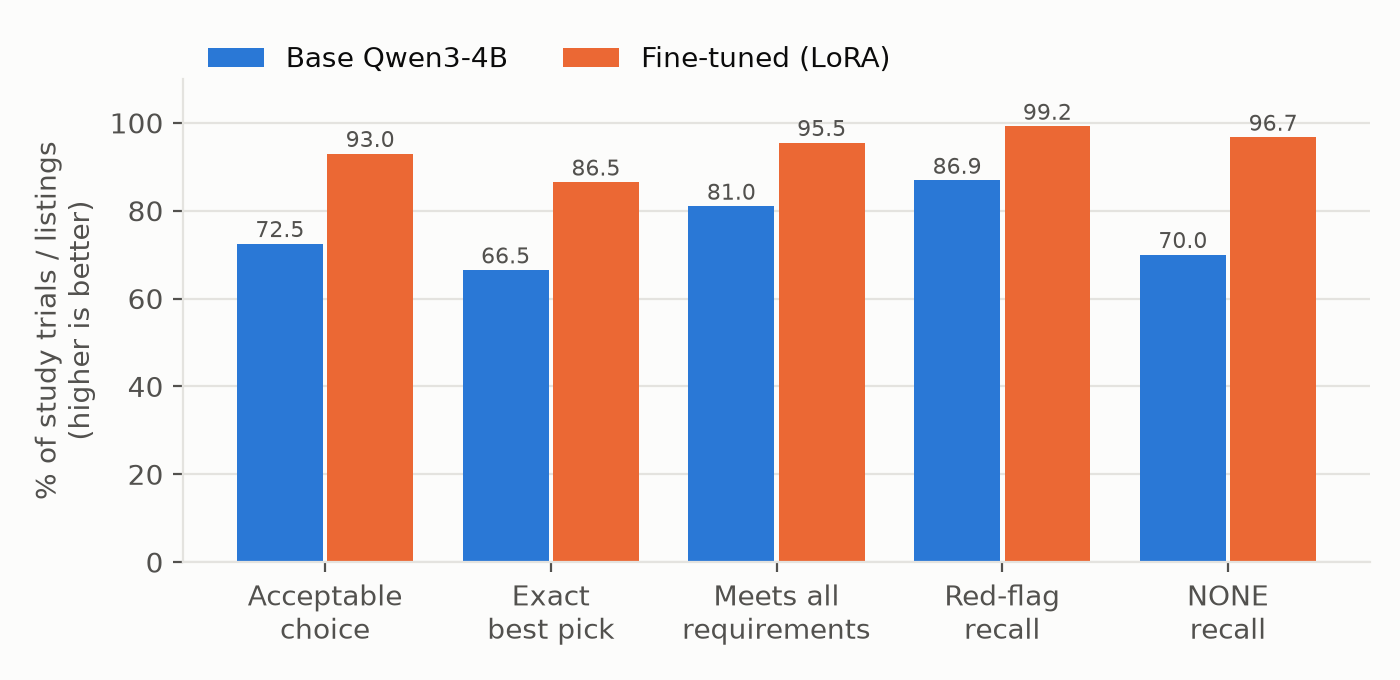
\includegraphics[width=0.8\linewidth]{../results/figures/base_vs_finetuned.png}
\caption{Before (base) and after (fine-tuned) on the main metrics. Higher is better for every metric shown.}
\label{fig:bars}
\end{figure}

\begin{table}[htbp]
\centering
\caption{Acceptable-choice rate by trial type and by wording (higher is better).}
\label{tab:subsets}
\begin{tabular}{lrrr}
\toprule
Subset & Trials & Base & Fine-tuned \\
\midrule
Clear & 30 & 90.0\% & 90.0\% \\
Trap & 70 & 72.9\% & 92.9\% \\
Trade-off & 70 & 65.7\% & 92.9\% \\
No suitable car & 30 & 70.0\% & 96.7\% \\
\midrule
Generated wording & 120 & 73.3\% & 94.2\% \\
Hand-written wording & 80 & 71.2\% & 91.2\% \\
\midrule
All & 200 & 72.5\% & 93.0\% \\
\bottomrule
\end{tabular}

\end{table}

Fine-tuning raised the acceptable-choice rate from \BaseAcc{} to \FtAcc{} and improved every
metric (Table~\ref{tab:metrics}, Figure~\ref{fig:bars}), which justifies fine-tuning in the first
place. Table~\ref{tab:subsets} breaks the acceptable-choice rate down by trial type and by wording,
to show \emph{where} fine-tuning helped and whether it holds up on text it never saw in training.
The largest gains are on the hard trial types: trap trials (72.9\% to 92.9\%), where
the base model often took the tempting car; trade-off trials, where it often picked a car another
qualifying car beats on both priorities (65.7\% to 92.9\%); and no-suitable-car trials (70.0\% to
96.7\%). On hand-written wording,
which never appears in training, the fine-tuned model scores \FtAccNatural{} versus
\FtAccTemplate{} on generated wording, so it generalizes to new phrasing with a small drop. Both
models score the same on clear trials, where every wrong car fails visibly.

\subsection{Error analysis}\label{sec:errors}

Following standard error-analysis practice \cite{errudite}, I first assign every wrong answer an
outcome category automatically (\gh{evaluate.py}{evaluate.py}): what went wrong. I then read each of the
\FtErrors{} fine-tuned errors by hand to find its root cause: why it went wrong
(\gh{results/ft_error_root_causes.csv}{results/ft\_error\_root\_causes.csv}). Figure~\ref{fig:errors} shows both distributions.

\begin{figure}[htbp]
\centering
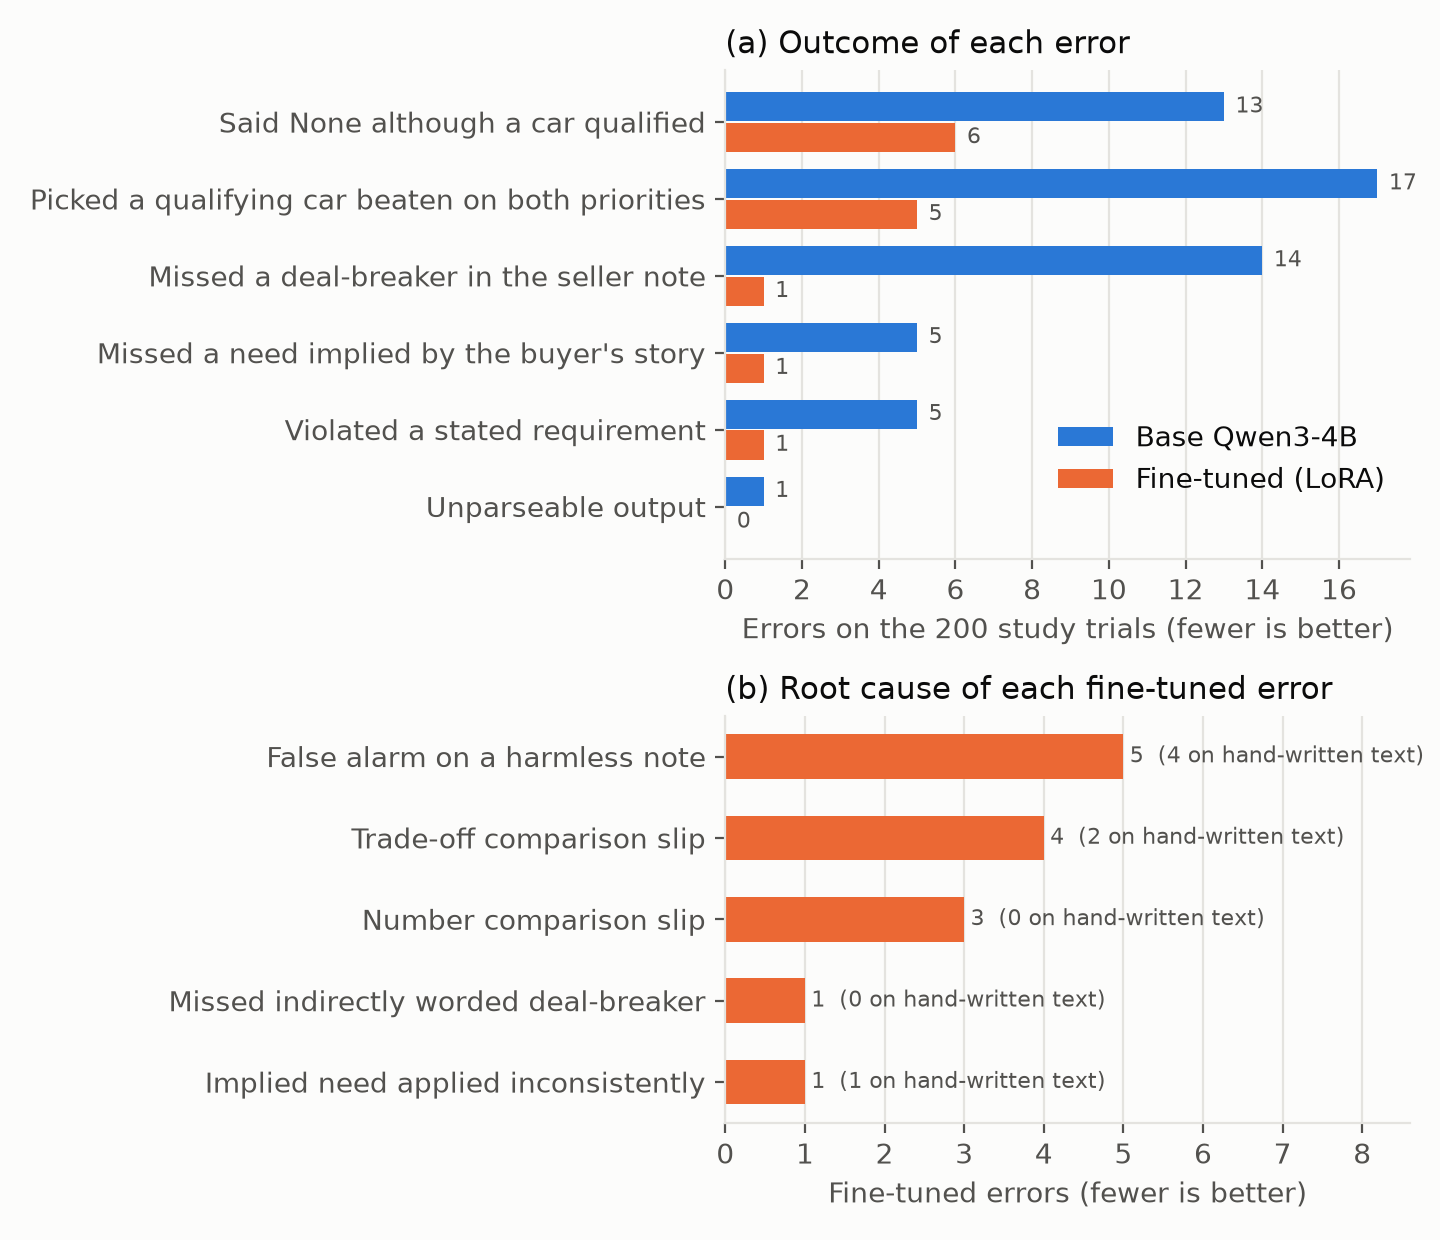
\includegraphics[width=0.86\linewidth]{../results/figures/error_analysis.png}
\caption{Error distributions. (a) Outcome category of every error, base vs.\ fine-tuned.
(b) Hand-labeled root cause of each fine-tuned error, with how many occurred on hand-written
wording. Bars count errors, so fewer is better.}
\label{fig:errors}
\end{figure}

\begin{table}[htbp]
\centering
\caption{Error distribution by outcome (automatic). Counts: lower is better. Percentages are
shares of each model's errors and describe the error mix, not better or worse.}
\label{tab:errors}
\begin{tabular}{lrr}
\toprule
Error pattern & Fine-tuned & Base \\
\midrule
Said None although a car qualified & 6 (42.9\%) & 13 (23.6\%) \\
Picked a qualifying car beaten on both priorities & 5 (35.7\%) & 17 (30.9\%) \\
Missed a deal-breaker in the seller note & 1 (7.1\%) & 14 (25.5\%) \\
Violated a stated requirement & 1 (7.1\%) & 5 (9.1\%) \\
Missed a need implied by the buyer's story & 1 (7.1\%) & 5 (9.1\%) \\
Unparseable output & 0 & 1 (1.8\%) \\
\midrule
Total errors (of 200 trials) & 14 & 55 \\
\bottomrule
\end{tabular}

\end{table}

\begin{table}[htbp]
\centering
\caption{Root causes of the \FtErrors{} fine-tuned errors (hand-labeled, one label per error).
Counts: lower is better; percentages are shares of the \FtErrors{} errors.}
\label{tab:rootcause}
\begin{tabularx}{\linewidth}{>{\raggedright\arraybackslash}p{0.25\linewidth}rrX}
\toprule
Root cause & Errors & \% of errors & Example from the study set \\
\midrule
False alarm on a harmless note & 5 & 35.7\% & ``Not a scam, I promise! Happy to meet at the
police station parking lot, bring your mechanic'' was flagged as a seller demanding payment
before any viewing (CAR-042); a DIY suspension rebuild was called ``title washing'' (CAR-192). \\
Trade-off comparison slip & 4 & 28.6\% & The model's own trade-off text says the alternative ``has
2,000 fewer miles'' in the same model year, the buyer's top two priorities, yet it recommends the
other car (CAR-152). \\
Number comparison slip & 3 & 21.4\% & ``All-in price \$10,199 is over the \$22,500 budget''
(CAR-165); an all-in price of \$11,699 called within an \$11,500 budget (CAR-038). \\
Missed an indirectly worded deal-breaker & 1 & 7.1\% & ``Some silt behind the dash panels from
when the river crested'' (flood damage) read as routine (CAR-059). \\
Implied need applied inconsistently & 1 & 7.1\% & The buyer's knee injury (``no clutch work'')
correctly ruled out one manual truck but not the other (CAR-180). \\
\midrule
Total & 14 & 100\% & \\
\bottomrule
\end{tabularx}
\end{table}

\paragraph{Reading the error tables:} Table~\ref{tab:errors} gives the exact counts behind
Figure~\ref{fig:errors}a. Fine-tuning cut errors from \BaseErrors{} to \FtErrors{}, and the mix
changed: missed seller-note deal-breakers, a quarter of the base model's errors (14), fell to one,
while unnecessary None answers became the fine-tuned model's largest error type (6 of 14).
Table~\ref{tab:rootcause} gives the counts behind Figure~\ref{fig:errors}b, with a real example of
each root cause from the study set; the two most common causes, false alarms and trade-off slips,
make up 9 of the 14 errors. The paragraphs below explain how each cause arises.

\paragraph{Overall pattern:} Fine-tuning changed \emph{how} the model fails. The base model mostly
made permissive errors: it accepted the tempting car with a hidden problem or a dominated
trade-off. The fine-tuned model rarely misses a deal-breaker (one miss in 200 trials) but has
become \emph{over-cautious}, and its remaining errors are small reasoning slips. The errors are
spread across trial types (3 clear, 5 trap, 5 trade-off, 1 no-suitable-car). When it is wrong, it
uses the same confident wording as when it is right (``Fails: \dots'' or ``Meets all
requirements'').

\paragraph{How each error happens and likely causes:}
\begin{itemize}
  \item \textbf{False alarms on harmless notes (5):} The model matches alarming words
  (``fender-bender'', ``rebuilt'', ``scam'', ``pothole'') to deal-breakers and sometimes invents a
  detail to justify it (``asks for payment before any viewing'' is not in the note). Four of the
  five are on hand-written notes. A likely cause is that training taught a strong link from damage
  and payment vocabulary to ``Fails'', and its harmless notes rarely used those words, so the model
  never learned the benign readings. The training mix may add to this: in trap trials the most
  attractive car always hides a problem, which can teach the model that attractive cars are
  suspicious.
  \item \textbf{Trade-off comparison slips (4):} In every case the model's own trade-off text
  states that the other car is better on the buyer's top priority. A likely cause is the output
  order: the JSON asks for the \code{recommendation} before the \code{tradeoffs}, so the model
  commits to a choice before it writes out the comparison. Small differences (1\,mpg, 2,000 miles)
  are also where small models are least reliable.
  \item \textbf{Number comparison slips (3):} The model computes the all-in price correctly but
  compares it with the wrong number, such as the car's own price instead of the budget, or reads
  \$11,699 as within \$11,500. These are typical of small language models, which handle numbers as
  text rather than calculating.
  \item \textbf{Indirectly worded deal-breaker (1):} ``Silt behind the dash from when the river
  crested'' requires an inference (silt + river = flood) that no training note phrased this way.
  \item \textbf{Inconsistent implied need (1):} The model checks each listing in a separate line
  with no consistency check across them, so the same inferred need (no clutch) was applied to one
  manual truck and not the other.
\end{itemize}

\paragraph{Can humans avoid these errors?} Mostly yes, which is the basis for expecting
complementarity:
\begin{itemize}
  \item \textbf{False alarms (5)} are visible: the AI quotes a reason the human can check against the
  note in a few seconds, and in several cases the stated reason is simply not in the note. Its
  wrong None answers are also conspicuous: an AI that rejects all four cars invites a second look.
  \item \textbf{Comparison slips (7)} are visible in the AI's own output. ``\$10,199 is over the
  \$22,500 budget'' is wrong at a glance, and in all four trade-off errors the AI's trade-off text
  itself states that the alternative is better.
  \item \textbf{The two remaining misses} (flood silt, the knee injury) depend on reading ordinary
  language carefully. People are good at this when they read closely, though a rushed participant
  could miss them too.
\end{itemize}
The risk is the reverse: a participant who trusts the AI's confident tone will accept these
errors, and one who distrusts it may override some of the \FtAcc{} of trials it gets right. These
are the over- and under-reliance effects studied in prior work \cite{bansal, bucinca}.

\subsection{Adjustments for human--AI complementarity}\label{sec:adjust}

\begin{table}[htbp]
\centering
\caption{Acceptable-choice rate across study-set iterations (same trials and answer key; only the
wording of 80 trials differs). Higher is better.}
\label{tab:iter}
\begin{tabular}{lrr}
\toprule
Study set & Base & Fine-tuned \\
\midrule
Iteration 1 (generated wording only) & 72.0\% & 92.5\% \\
Iteration 2 (final, 40\% hand-written) & 72.5\% & 93.0\% \\
\bottomrule
\end{tabular}

\end{table}

\paragraph{What I changed and why:} Two results drove my adjustments. First, the base model alone
(\BaseAcc{}) was too weak to be useful assistance, so I fine-tuned it (Part~\ref{part:model}). I
also made the output parser tolerant of the base model's formatting quirks, so its score reflects
its decisions rather than its formatting. Second, on the template-only iteration-1 study set the
fine-tuned model scored \FtAccOne{}, close to the point where people should simply delegate, so I
added hand-written wording to 40\% of the study set (Section~\ref{sec:data}). The overall score
barely moved (Table~\ref{tab:iter}), but the model's remaining errors now cluster on exactly the
kinds of text where human reading should help: alarming-but-harmless notes and indirect wording.
That is what makes complementarity possible.

\paragraph{Why the study set is balanced, and why that matters after fine-tuning:} The study set is
not skewed toward one type of trial: 30 clear, 70 trap, 70 trade-off and 30 no-suitable-car trials;
40 trials per buyer type; correct answers spread across A--D and None (A 40, B 44, C 48, D 38,
None 30); and 60\% generated vs.\ 40\% hand-written wording. This matters because the AI's and the
humans' weaknesses sit in different trial types:
\begin{itemize}
  \item People are likely to struggle on \emph{trap} and \emph{trade-off} trials, where the problem
  hides in fine print or requires arithmetic. The fine-tuned AI is strong there.
  \item The fine-tuned AI's errors are over-caution (wrong None answers, false alarms) and slips in
  close comparisons, which plain reading catches.
\end{itemize}
A set skewed toward clear trials would leave everyone near the ceiling, with nothing to
complement; a set skewed toward traps would make the AI look nearly perfect and invite
delegation. Balancing the answer letters also prevents participants or the model from scoring
well by favoring one position, and including None trials tests whether people notice when the AI
should, or should not, reject every car.

\paragraph{What I did not change:} I considered making the task harder so the AI would score
lower, but decided against it: the remaining AI errors are confident, varied and catchable by
humans, which is the complementarity I want to test, and the task should keep a realistic mix of
easy and hard trials.

\subsection{Prediction}\label{sec:prediction}

\textbf{I predict: Human+AI $>$ AI-only $>$ Human-only}, measured by how often the chosen car is
an acceptable choice. The AI and the person make different kinds of mistakes, and each is good
at what the other gets wrong, so together they should do better than either one alone.

\begin{itemize}
  \item \textbf{Human+AI: highest, roughly 93--97\%:} This range is an estimate that assumes
  participants actually check the AI's reasons against the listings; without that checking, Human+AI
  would land at or below the AI's \FtAcc{} (see the risks below). The AI helps with what people tend to get
  wrong in a hurry: it adds up the fees, checks every requirement for every car, compares the cars
  on the buyer's two priorities, and spots deal-breakers hidden in seller notes (it caught
  \FtFlagRecall{} of them). The person helps with what the AI gets wrong. My error analysis
  (Section~\ref{sec:errors}) shows that 12 of the AI's \FtErrors{} mistakes can be seen just by
  reading its answer. When it wrongly rejects a car, the reason it gives is often not in the note.
  When it compares numbers wrongly, the mistake is obvious (``\$10,199 is over the \$22,500
  budget''). When it says no car works, that alone makes people look again. These mistakes
  happen mostly on harmless notes that sound alarming and on casual wording, which people read
  well.
  \item \textbf{AI-only: \FtAcc{}} (measured, Table~\ref{tab:metrics}). Good, but it cannot catch
  its own mistakes: it sounds just as sure when it is wrong as when it is right.
  \item \textbf{Human-only: lowest, roughly 60--75\%:} In 2--3 minutes per trial, a person has
  to check four cars against up to seven requirements, spot fees mentioned only in the fine print,
  work out needs the buyer only hints at, and compare the cars on both of the buyer's priorities to
  rule out any car that another one beats on both. The trap, trade-off and no-suitable-car trials
  are built around exactly the checks people skip when rushed, and many classmates may not know
  warning signs such as a ``washed'' title or a seller asking you to pay through an ``eBay agent''.
  I expect people to do well on clear trials and on obvious red flags, and worse on fees, hinted
  needs and trade-offs.
\end{itemize}

\paragraph{What could make this prediction wrong:} The AI is already right on \FtAcc{} of trials,
so there is little room to beat it (only \FtErrors{} mistakes in 200 trials). Past studies found
that when the AI is much better than people, showing its reasons can make people simply agree
with it more, instead of catching its mistakes \cite{bansal, bucinca}. Human+AI only beats the AI
alone if people fix more of its mistakes than they create by overruling its correct answers. Two
things work against this: people trusting the AI when it is confidently wrong, and people
ignoring the AI when it correctly rejects a car that looks like a good deal. To help, participants
see the AI's reasons, not just its pick, so they can check each claim against the listing.
Either way, Human+AI should do much better than a person alone.

% ===========================================================================
\phantomsection
\section*{Study guidelines and participant expectations (Assignment 3)}\label{sec:guidelines}
\addcontentsline{toc}{section}{Study guidelines and participant expectations}

This section describes what participants will see and do in the user study.

\paragraph{What the participant is given:}
\begin{itemize}
  \item A \textbf{buyer profile} in plain language: who the buyer is, an all-in budget (price plus
  any required dealer fees), hard requirements, and two soft priorities (for example, ``low miles
  first, then price''). Some requirements are stated outright (``It has to be an automatic'');
  others are only implied by the story (``I never learned to drive stick'', ``we have three kids
  and my parents ride along most weekends'').
  \item \textbf{Four listings (A--D)}, each with year, make, model, price, mileage, body style,
  seats, drivetrain, transmission, fuel economy, title status, seller type and location, plus a
  free-text \textbf{seller note}.
  \item In the \textbf{AI-assisted condition}, also the AI's recommendation, its check of each
  listing, the red flags it found, its reason and its stated trade-offs
  (Section~\ref{sec:assist}).
\end{itemize}

\paragraph{What the participant must do:} Choose A, B, C, D or None, and briefly explain why. After
each choice I will also ask, without scoring it, how confident they are and whether they would
actually buy that car. Each trial takes about 2--3 minutes, so a participant completes 3--4 trials
in a 10-minute session.

\paragraph{How answers are scored:} With the same rules as the AI (Section~\ref{sec:bench}): a
choice is correct if it meets every requirement and no other qualifying car is better on both
priorities, or if it is None when nothing qualifies.

\paragraph{Planned trial selection:} With approximately 70 classmates, I expect roughly 210--280 completed
trials. Rather than spreading them over all 200, I plan to use a balanced subset of about 40--60
trials (all trial types, both wordings, and some of the AI's errors) so that each trial receives
several answers in each condition and human-only and human+AI can be compared on the same trials.

\begin{trialbox}{Example trial CAR-131 (trap, hand-written wording), abridged}
\small
\textbf{Buyer:} ``I work early shifts, so I'm often driving before the plows have been out. I can
spend at most \$25,000 total, including any required dealer fees. It needs all-wheel or
four-wheel drive. I can't afford surprises, so no hidden damage, no questionable title or mileage
history, no scam-like sellers, and no big repairs looming. Within those limits, what I care about
most is getting something newer, and after that as few miles as possible.''

\smallskip
\begin{tabularx}{\linewidth}{@{}l>{\raggedright\arraybackslash}p{0.36\linewidth}X@{}}
\toprule
& Listing & Seller note \\
\midrule
A & 2013 Hyundai Elantra, \$2,500, 206,500 mi, FWD & ``Check engine light came on once, turned out to be a loose gas cap.'' \\
B & 2020 Subaru Ascent, \$17,400, 43,500 mi, AWD & ``Priced well below KBB because I need it gone before I leave the country Friday. eBay Motors protection: you pay through their agent and get 5 days to inspect after delivery.'' \\
C & 2023 Toyota Sienna, \$28,400, 22,000 mi, AWD & ``Ate a pothole and needed a new tire and rim last winter.'' \\
D & 2015 Honda Pilot, \$7,400, 157,500 mi, AWD & ``Water pump and timing belt were replaced at 95k as recommended.'' \\
\bottomrule
\end{tabularx}

\smallskip
\textbf{Correct answer: D.} A is front-wheel drive and C is over budget, both visible in the
fields. B is the trap: it is the newest affordable AWD car, but paying a stranger's ``agent''
before seeing the car is a well-known online car-sale scam. Only D meets every requirement.
The base model recommended B; the fine-tuned model flagged B as a scam and recommended D.
\end{trialbox}


% ===========================================================================
\section*{Appendix: submitted files and how to reproduce}
\addcontentsline{toc}{section}{Appendix: submitted files}

The Canvas submission has two zips. \path{CSE594_A2_car_advisor_files.zip} contains this
report and the \code{car\_advisor/} folder with everything except the trained adapter;
\path{CSE594_A2_car_advisor_adapter.zip} contains only the adapter and unzips into the same
folder. The same files, including the adapter, are in the GitHub repository, where the adapter is
stored as two zip parts that \gh{setup.sh}{setup.sh} rebuilds:\\ \url{https://github.com/rajdeeepm/ai-car-advisor}\\
The \gh{README.md}{README.md} has full instructions, and the file names below link to the repository.

\begin{tabularx}{\linewidth}{>{\raggedright\arraybackslash}p{0.38\linewidth}X}
\toprule
File & Contents \\
\midrule
\gh{submission/study_dataset.csv}{submission/study\_dataset.csv} & \textbf{Study dataset, 200 trials}: buyer profile and listings
A--D (input); model choice, red flags, reason, trade-offs and raw output (model output);
per-listing issues, qualifying options, acceptable and best answers, correctness and error
category (evaluation); base-model columns for comparison \\
\gh{submission/participant_trials.csv}{submission/participant\_trials.csv} & Participant view for Assignment 3 (no answer key) \\
\gh{data/train.jsonl}{data/train.jsonl}, \gh{data/val.jsonl}{data/val.jsonl} & Training (1,620) and validation (180) data \\
\gh{data/study.jsonl}{data/study.jsonl}, \gh{data/study_v1.jsonl}{data/study\_v1.jsonl} & Final study set and the iteration-1 version \\
\gh{gen_dataset.py}{gen\_dataset.py}, \gh{natural_text.py}{natural\_text.py}, \gh{make_study_v2.py}{make\_study\_v2.py} & Dataset generation \\
\gh{prompts.py}{prompts.py}, \gh{train_lora.py}{train\_lora.py}, \gh{infer.py}{infer.py}, \gh{demo.py}{demo.py}, \gh{run_all.sh}{run\_all.sh} &
Model training and inference \\
\gh{evaluate.py}{evaluate.py}, \gh{make_report_assets.py}{make\_report\_assets.py}, \gh{export_csv.py}{export\_csv.py} & Metrics, error analysis,
report tables and figures \\
\gh{results/ft_error_root_causes.csv}{results/ft\_error\_root\_causes.csv} & Hand-labeled root cause of each fine-tuned error \\
\ghdir{preds}{preds/}, \ghdir{results}{results/} & Saved raw model outputs and scores for both iterations \\
\ghdir{model}{model/lora\_adapter/}, \gh{model/log_history.json}{model/log\_history.json}, \gh{setup.sh}{setup.sh} & Trained LoRA adapter (split zip in the repository; \code{setup.sh} rebuilds it) and training log \\
\gh{report/report.tex}{report/report.tex} & Source of this report \\
\bottomrule
\end{tabularx}

\paragraph{Reproducing the reported numbers (no GPU, seconds):} These commands rebuild every table,
figure and number in this report from the saved model outputs:
\begin{Verbatim}[fontsize=\small]
python evaluate.py --preds preds/base_study.jsonl preds/ft_study.jsonl
python make_report_assets.py
\end{Verbatim}

\paragraph{Reproducing everything:} The first command regenerates all data byte-for-byte from the
seeds; the second retrains the adapter and regenerates all predictions on one GPU (about 40
minutes):
\begin{Verbatim}[fontsize=\small]
python gen_dataset.py --out data && cp data/study.jsonl data/study_v1.jsonl && python make_study_v2.py
MODEL=<path to Qwen3-4B-Instruct-2507> bash run_all.sh
\end{Verbatim}

\begin{thebibliography}{9}
\bibitem{qwen3} Qwen Team. \emph{Qwen3 Technical Report}. arXiv:2505.09388, 2025.
\bibitem{lora} E.~J. Hu, Y.~Shen, P.~Wallis, Z.~Allen-Zhu, Y.~Li, S.~Wang, L.~Wang, W.~Chen.
\emph{LoRA: Low-Rank Adaptation of Large Language Models}. ICLR, 2022.
\bibitem{bansal} G.~Bansal, T.~Wu, J.~Zhou, R.~Fok, B.~Nushi, E.~Kamar, M.~T. Ribeiro, D.~Weld.
\emph{Does the Whole Exceed its Parts? The Effect of AI Explanations on Complementary Team
Performance}. CHI, 2021.
\bibitem{bucinca} Z.~Bu\c{c}inca, M.~B. Malaya, K.~Z. Gajos. \emph{To Trust or to Think: Cognitive
Forcing Functions Can Reduce Overreliance on AI in AI-assisted Decision-making}. CSCW, 2021.
\bibitem{errudite} T.~Wu, M.~T. Ribeiro, J.~Heer, D.~Weld. \emph{Errudite: Scalable, Reproducible,
and Testable Error Analysis}. ACL, 2019.
\end{thebibliography}

\end{document}
